% IE4483 Mini Project (Option 2): Dogs vs. Cats. Team 97.
% Compile with pdfLaTeX and BibTeX (the Overleaf defaults).
\documentclass[11pt,a4paper]{article}

\usepackage[T1]{fontenc}
\usepackage{mathptmx}   % Times text and maths, much faster to load than newtx
\usepackage{amssymb}
\renewcommand{\ttdefault}{lmtt}   % vector typewriter font for code and file names
\usepackage[a4paper,margin=2.3cm]{geometry}
\usepackage{microtype}
\usepackage{graphicx}
\usepackage{booktabs}
\usepackage{tabularx}
\usepackage{array}
\usepackage{amsmath}
\usepackage{xcolor}
\usepackage{enumitem}
\usepackage[section]{placeins}
\usepackage[font=small,labelfont=bf,labelsep=period]{caption}
\usepackage[numbers,square,sort&compress]{natbib}
\PassOptionsToPackage{hyphens}{url}   % long URLs may break at hyphens, so bibliography lines fit
\usepackage[colorlinks=true,linkcolor=blue!50!black,citecolor=blue!50!black,urlcolor=blue!50!black]{hyperref}
\usepackage[capitalise,noabbrev]{cleveref}

% Sections are labelled (a) to (h) to match the questions in the project brief.
\renewcommand{\thesection}{(\alph{section})}
\crefname{section}{Section}{Sections}

\setlength{\parskip}{0.45em}
\setlength{\parindent}{0pt}
\setlength{\emergencystretch}{2em}
\setlist{itemsep=0.15em,topsep=0.3em}

% Question from the brief, quoted at the start of each section.
\newsavebox{\questionbox}
\newenvironment{question}
  {\par\smallskip\noindent\begin{lrbox}{\questionbox}%
   \begin{minipage}{\dimexpr\linewidth-2\fboxsep-2\fboxrule\relax}\small\itshape}
  {\end{minipage}\end{lrbox}%
   \fcolorbox{gray!45}{gray!7}{\usebox{\questionbox}}\par\smallskip}
\setlength{\fboxsep}{5pt}
\setlength{\fboxrule}{0.4pt}

\newcommand{\pct}[1]{#1\%}
\newcommand{\pmpct}[2]{$#1 \pm #2$\%}
\newcommand{\pdog}{$p(\mathrm{dog})$}
\newcommand{\repo}{\url{https://github.com/Dheemant19/IE4483-Team97}}


\begin{document}

% ------------------------------------------------------------------ title
\begin{center}
  {\Large\bfseries IE4483 Artificial Intelligence and Data Mining\par}
  \vspace{0.4em}
  {\LARGE Dogs vs.\ Cats Project Report\par}
  \vspace{0.4em}
  {\large Mini Project (Option 2), Team 97\par}
\end{center}

\vspace{0.6em}
\begin{table}[ht]
  \centering
  \small
  \begin{tabularx}{\textwidth}{@{}l l l >{\raggedright\arraybackslash}X@{}}
    \toprule
    Name & Matriculation No. & Email & Contribution \\
    \midrule
    Nicole Lim Xin En      & U2323352G & \href{mailto:NLIM064@e.ntu.edu.sg}{NLIM064@e.ntu.edu.sg} & Report writing and analysis for parts (a) to (d). \\
    Dheemant Rastogi       & U2323523J & \href{mailto:dheemant001@e.ntu.edu.sg}{DHEEMANT001@e.ntu.edu.sg} & Model implementation, data pre-processing, training, experimentation, result generation, figures and testing. \\
    Fok Jing Wei, Ernest   & U2321584D & \href{mailto:EFOK001@e.ntu.edu.sg}{EFOK001@e.ntu.edu.sg} & Report writing and analysis for parts (e) to (h). \\
    \bottomrule
  \end{tabularx}
\end{table}

{\centering\small Code, settings and results of all experiments: \repo\par}

\vspace{-0.5em}
{\small\tableofcontents}

\clearpage

% ================================================================== (a)
\section{Data and Pre-processing}\label{sec:a}

\begin{question}
State the amount of image data that you used to form your training set and testing set. Describe the data pre-processing procedures and image augmentations (if any).
\end{question}

\subsection*{Dataset}

The Dogs vs.\ Cats dataset~\cite{kaggle2013} provided for this project consists of 25,500 images split into training, validation, and testing sets (\cref{tab:dataset}). All 20,000 training images were used. The validation set originally had 5,000 images, but an MD5 hash check revealed that one cat image (\texttt{val/cat/cat.12408.jpg}) was an exact duplicate of a training image (\texttt{train/cat/cat.2339.jpg}). This duplicate was removed to prevent data leakage, leaving 4,999 validation images. The same check also found four more groups of identical images within the training set (three pairs and one group of three), which were kept because they do not affect validation accuracy. The 500 unlabelled testing images were used only for the final predictions and not for model selection. Following the submission format, cats were labelled as 0 and dogs as 1.

\begin{table}[ht]
  \centering
  \small
  \caption{Distribution of images across the training, validation and testing sets.}
  \label{tab:dataset}
  \begin{tabular}{@{}lrrrl@{}}
    \toprule
    Set & Cat images & Dog images & Total & Used for \\
    \midrule
    Training   & 10,000 & 10,000 & 20,000 & optimising the model weights \\
    Validation &  2,499 &  2,500 &  4,999 & model selection and all reported accuracies \\
    Testing    &     -- &     -- &    500 & \texttt{submission.csv} only \\
    \bottomrule
  \end{tabular}
\end{table}

The images vary widely in resolution and aspect ratio (\cref{fig:sizes}). Across the 25,499 retained images, the shorter side ranges from 32 to 768 pixels (median of 366 pixels), and the longest side reaches 1,050 pixels. In total, 208 images have a shorter side below 100 pixels, and 3,015 images (\pct{11.8}) have a shorter side below 224 pixels.

\begin{figure}[ht]
  \centering
  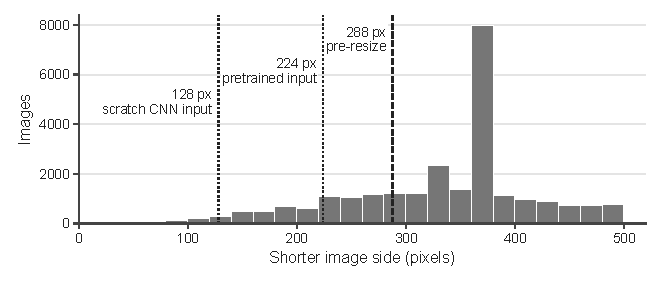
\includegraphics[width=0.78\textwidth]{figures/image_sizes.pdf}
  \caption{Distribution of the shorter image side over all 25,499 images (20-pixel bins).}
  \label{fig:sizes}
\end{figure}

\subsection*{Data Pre-processing}

Several models were compared in this project, including a convolutional neural network (CNN) trained from scratch and a set of pretrained models, from which DINOv2-B was selected as the final model. \Cref{sec:b} introduces the models, and \cref{sec:f} gives the details of the scratch CNN and the classical baselines. The input sizes of these models shaped the pre-processing below.

Before training, all images were converted to RGB format to keep the input data consistent. Because the original images varied in resolution and aspect ratio, a preliminary resizing step was performed to speed up data loading. Images with a shorter side above 288 pixels were downscaled so that this side became 288 pixels, keeping the original aspect ratio. This affected 18,771 images (\pct{73.6}). Images with a shorter side of 288 pixels or less were not resized in this step, to avoid unnecessary upscaling. The resized copies were stored as JPEG files at quality 95, which made image decoding 1.38 times faster on the training server.

The images were then resized and cropped to the input size of each model. The pretrained models used $224 \times 224$ pixels (except EfficientNetV2-S, which used $300 \times 300$ pixels), and the scratch CNN and the classical baselines used $128 \times 128$ pixels. Since the 288-pixel threshold lies above the 224-pixel input of the final model (\cref{fig:sizes}), the preliminary resizing does not limit the resolution available to it. Only EfficientNetV2-S received images that had been reduced to 288 pixels and then slightly enlarged again to 300 pixels.

For validation and testing, a deterministic procedure was applied. The shorter side of each image was resized to a fixed length set by the model's default crop ratio (224 pixels for DINOv2-B, with bicubic interpolation), and the central square of the input size was then cropped. The images were converted into tensors and normalised with each model's channel-wise mean and standard deviation. The pretrained models used their specified values (the ImageNet statistics for DINOv2-B), and the scratch CNN used statistics computed on the training set.

\subsection*{Image Augmentation}

Image augmentation was applied during training to add variation to the images and help the models generalise to unseen data. The default augmentation pipeline included random resized cropping, horizontal flipping, rotation, colour jitter and random erasing~\cite{zhong2020erasing}.

For the pretrained models, random resized cropping selected between \pct{50} and \pct{100} of the image area, with an aspect ratio between 3/4 and 4/3. The scratch CNN used a range of \pct{60} to \pct{100}. Horizontal flipping was applied with a probability of 0.5, and random rotation was performed within $\pm 15^\circ$. Colour jitter varied brightness, contrast and saturation by factors between 0.8 and 1.2 and shifted the hue by up to 0.02 of the colour wheel. Random erasing was applied with a probability of 0.25 to simulate partial obstruction.

\Cref{fig:aug} shows the stored image (shorter side of 288 pixels), the deterministic validation and test input and five random draws of the training transform for a cat and a dog image. The grey rectangles come from random erasing, which fills them with the ImageNet mean colour, and the black corners are empty regions left by rotation.

\begin{figure}[ht]
  \centering
  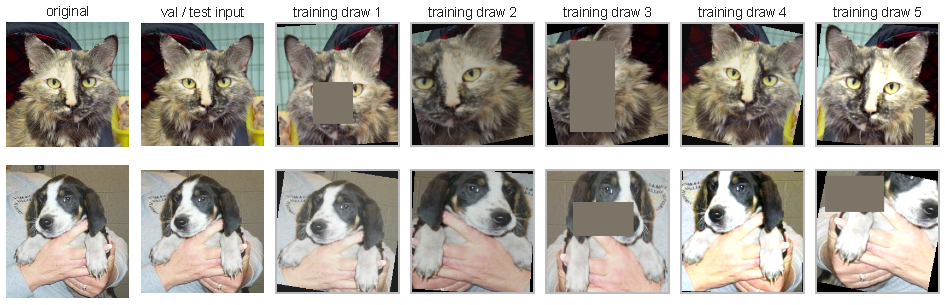
\includegraphics[width=\textwidth]{figures/aug_examples.pdf}
  \caption{Examples of pre-processing and augmentation for the pretrained models.}
  \label{fig:aug}
\end{figure}

These techniques varied the position, orientation and appearance of the cats and dogs, which helped the models learn features that depend less on specific image conditions. Their effect is measured in \cref{sec:f}, where the scratch CNN, which has no pretrained features, benefits the most. Random augmentations were not applied to the validation and testing sets. However, horizontal-flip test-time augmentation (TTA) was used at prediction time, which averages the predictions for the original and the horizontally flipped image. The final model uses it (\cref{fig:pipeline}), and \cref{tab:models} reports each neural network with and without it.

% ================================================================== (b)
\section{Model, Training Strategy and Code}\label{sec:b}

\begin{question}
Select or build at least one machine learning model (e.g., CNN + linear layer, etc.) to construct your classifier. Clearly describe the model you use, including a figure of model architecture, the input and output dimensions, structure of the model, loss function(s), training strategy, etc. Include your code and instructions on how to run the code. If non-deterministic method is used, ensure reproducibility of your results by averaging the results over multiple runs, cross-validation, fixing random seed, etc.
\end{question}

\subsection*{Model Selection}

Several machine learning models were evaluated for the Dogs vs.\ Cats task. These were two classical baselines of histogram of oriented gradients (HOG) features with a support vector machine (SVM)~\cite{dalal2005hog,cortes1995svm}, a CNN trained from scratch, and the pretrained models ResNet-50~\cite{he2016resnet}, EfficientNetV2-S~\cite{tan2021efficientnetv2}, ConvNeXt-T~\cite{liu2022convnext} and DINOv2~\cite{oquab2024dinov2} in its small (S) and base (B) sizes. Based on the validation results, DINOv2-B was selected as the final model. Used as a linear probe (described below), it reached a mean validation accuracy of \pmpct{99.86}{0.02}, against \pct{97.65} for the scratch CNN and \pct{80.06} for the best SVM. This was the highest of all models in the full comparison of \cref{sec:f}.

DINOv2-B is a pretrained Vision Transformer (ViT-B/14)~\cite{dosovitskiy2021vit} that learns visual features through self-supervised pretraining on LVD-142M, a curated collection of 142 million unlabelled images~\cite{oquab2024dinov2}. In this project, the model was used as a frozen feature extractor with an added linear classification layer, an approach known as linear probing. Instead of retraining the whole network, only this layer was trained to separate cats from dogs. This reduces the number of trainable parameters while making use of the visual features that the model has already learned.

\subsection*{Model Architecture}

The DINOv2-B model takes an RGB image of $3 \times 224 \times 224$ pixels as input (\cref{fig:arch,tab:arch}). Each image is divided into 256 non-overlapping patches of $14 \times 14$ pixels, arranged in a $16 \times 16$ grid. A $14 \times 14$ convolution with stride 14 converts these patches into 768-dimensional feature embeddings. A classification token ([CLS]) is added, giving 257 tokens in total, and learned position embeddings are added to every token. The model was pretrained at $518 \times 518$ pixels, so its position embeddings were interpolated to the $16 \times 16$ grid. The tokens then pass through 12 transformer blocks, which extract visual features from the image. Each block consists of multi-head self-attention and a multilayer perceptron with residual connections.

After a final layer normalisation, the output of the [CLS] token is a 768-dimensional feature vector $\mathbf{h}$. This vector is passed into a linear classification layer with two output neurons, $\mathbf{z} = W\mathbf{h} + \mathbf{b}$ with $W \in \mathbb{R}^{2 \times 768}$. The softmax function converts the resulting logits into class probabilities, $p_c = e^{z_c} / (e^{z_0} + e^{z_1})$, where class index 0 is a cat and index 1 is a dog.

The model has about 85.73 million parameters (85,726,466). However, since the pretrained backbone was frozen during training, only the 1,538 parameters of the final linear layer ($768 \times 2$ weights and 2 biases) were updated.

In \cref{fig:arch}, the patch grid is drawn as $4 \times 4$ for clarity, whereas the model uses $16 \times 16$ patches, and the softmax values illustrate a confident prediction for a dog image. \Cref{tab:arch} lists the output shape and parameter count of each stage. A full layer-by-layer table is available in the project repository (\texttt{report/model\_summaries/dinov2\_b\_probe.txt}).

\begin{figure}[ht]
  \centering
  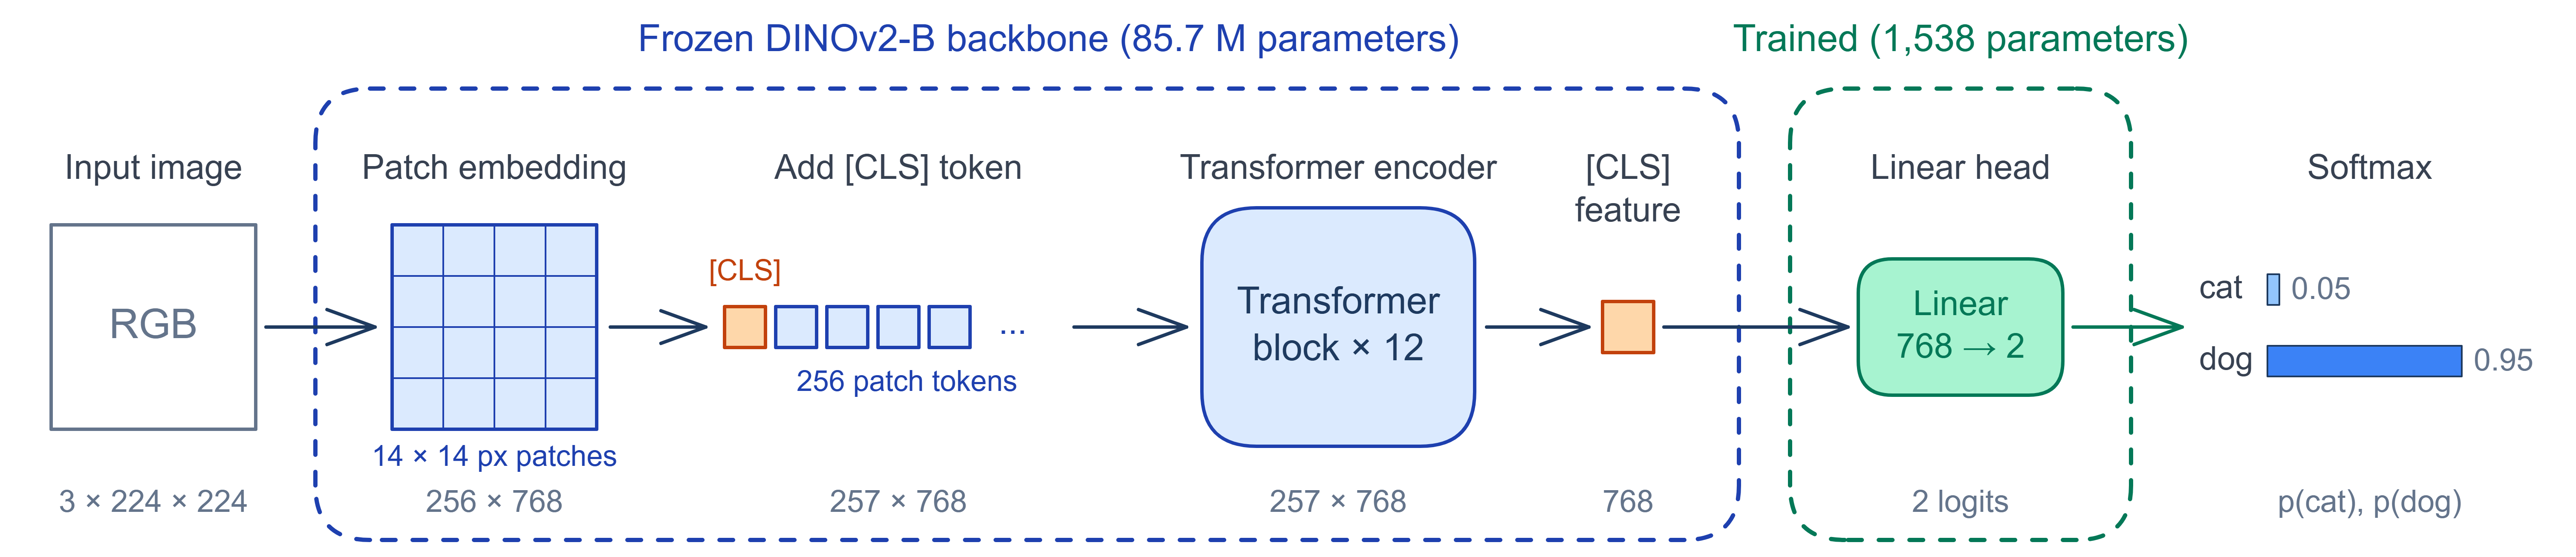
\includegraphics[width=\textwidth]{figures/arch_dinov2_probe.png}
  \caption{Architecture of the DINOv2-B classification model.}
  \label{fig:arch}
\end{figure}

\begin{table}[ht]
  \centering
  \small
  \caption{Output shape and parameter count of each stage of the final model. $B$ is the batch size (64 images during training).}
  \label{tab:arch}
  \begin{tabular}{@{}llrc@{}}
    \toprule
    Stage & Output shape & Parameters & Trained \\
    \midrule
    Input image (RGB)                                   & $B \times 3 \times 224 \times 224$ & -- & -- \\
    Patch embedding ($14 \times 14$ convolution, stride 14) & $B \times 256 \times 768$ & 452,352 & no \\
    {[CLS]} token and position embeddings               & $B \times 257 \times 768$ & 198,144 & no \\
    12 transformer blocks                               & $B \times 257 \times 768$ & 85,072,896 & no \\
    Final layer normalisation, [CLS] output             & $B \times 768$ & 1,536 & no \\
    Linear head                                         & $B \times 2$ & 1,538 & yes \\
    Softmax                                             & $B \times 2$ & -- & -- \\
    \midrule
    Total                                               &     & 85,726,466 & 1,538 \\
    \bottomrule
  \end{tabular}
\end{table}

\subsection*{Model Training}

The model was trained with cross-entropy loss and label smoothing of 0.1~\cite{szegedy2016labelsmoothing} to reduce overconfident predictions. With smoothing factor $\varepsilon = 0.1$ and true class $y$, the loss for one image is
\begin{equation}
  \mathcal{L} = -\sum_{c \in \{0,1\}} q_c \log p_c, \qquad
  q_c = (1 - \varepsilon)\,\mathbf{1}[c = y] + \frac{\varepsilon}{2},
  \label{eq:loss}
\end{equation}
so the targets are 0.95 for the true class and 0.05 for the other class. The AdamW optimiser~\cite{loshchilov2019adamw} was used with a learning rate of 0.001 for the classification layer and a weight decay of 0.05, which was not applied to the bias terms. Training ran for 10 epochs with a batch size of 64. The learning rate followed a one-epoch linear warm-up~\cite{goyal2017warmup} and then a cosine decay~\cite{loshchilov2017sgdr}. The reported results come from the model at the last training epoch, because choosing the epoch with the highest validation accuracy would give an optimistically biased estimate.

The training curves of the final model are shown in \cref{sec:c}, where they are compared with the alternative fine-tuning strategy (\cref{fig:curves}).

\subsection*{Reproducibility and Final Prediction}

To make the results more reliable, the model was trained three times, with the random seeds 0, 1 and 2. The seed fixes the random choices in training, such as the initial weights of the head and the order of the training images. However, GPU computations are not fully deterministic, so repeating a run with the same seed can still change the result slightly (by up to 0.05 percentage points for the pretrained models). Results are therefore reported as the mean and standard deviation over seeds. Throughout this report, the column $n$ in the tables gives the number of seeds, which is three unless stated otherwise.

For the final classifier, the three seed models were combined into an ensemble, and each was applied with flip TTA (\cref{sec:a}). Each test image therefore receives six dog-class probabilities, and their mean \pdog\ is compared with a threshold of 0.5 (\cref{fig:pipeline}). The ensemble reduces the dependence of the final predictions on any individual training run.

\begin{figure}[ht]
  \centering
  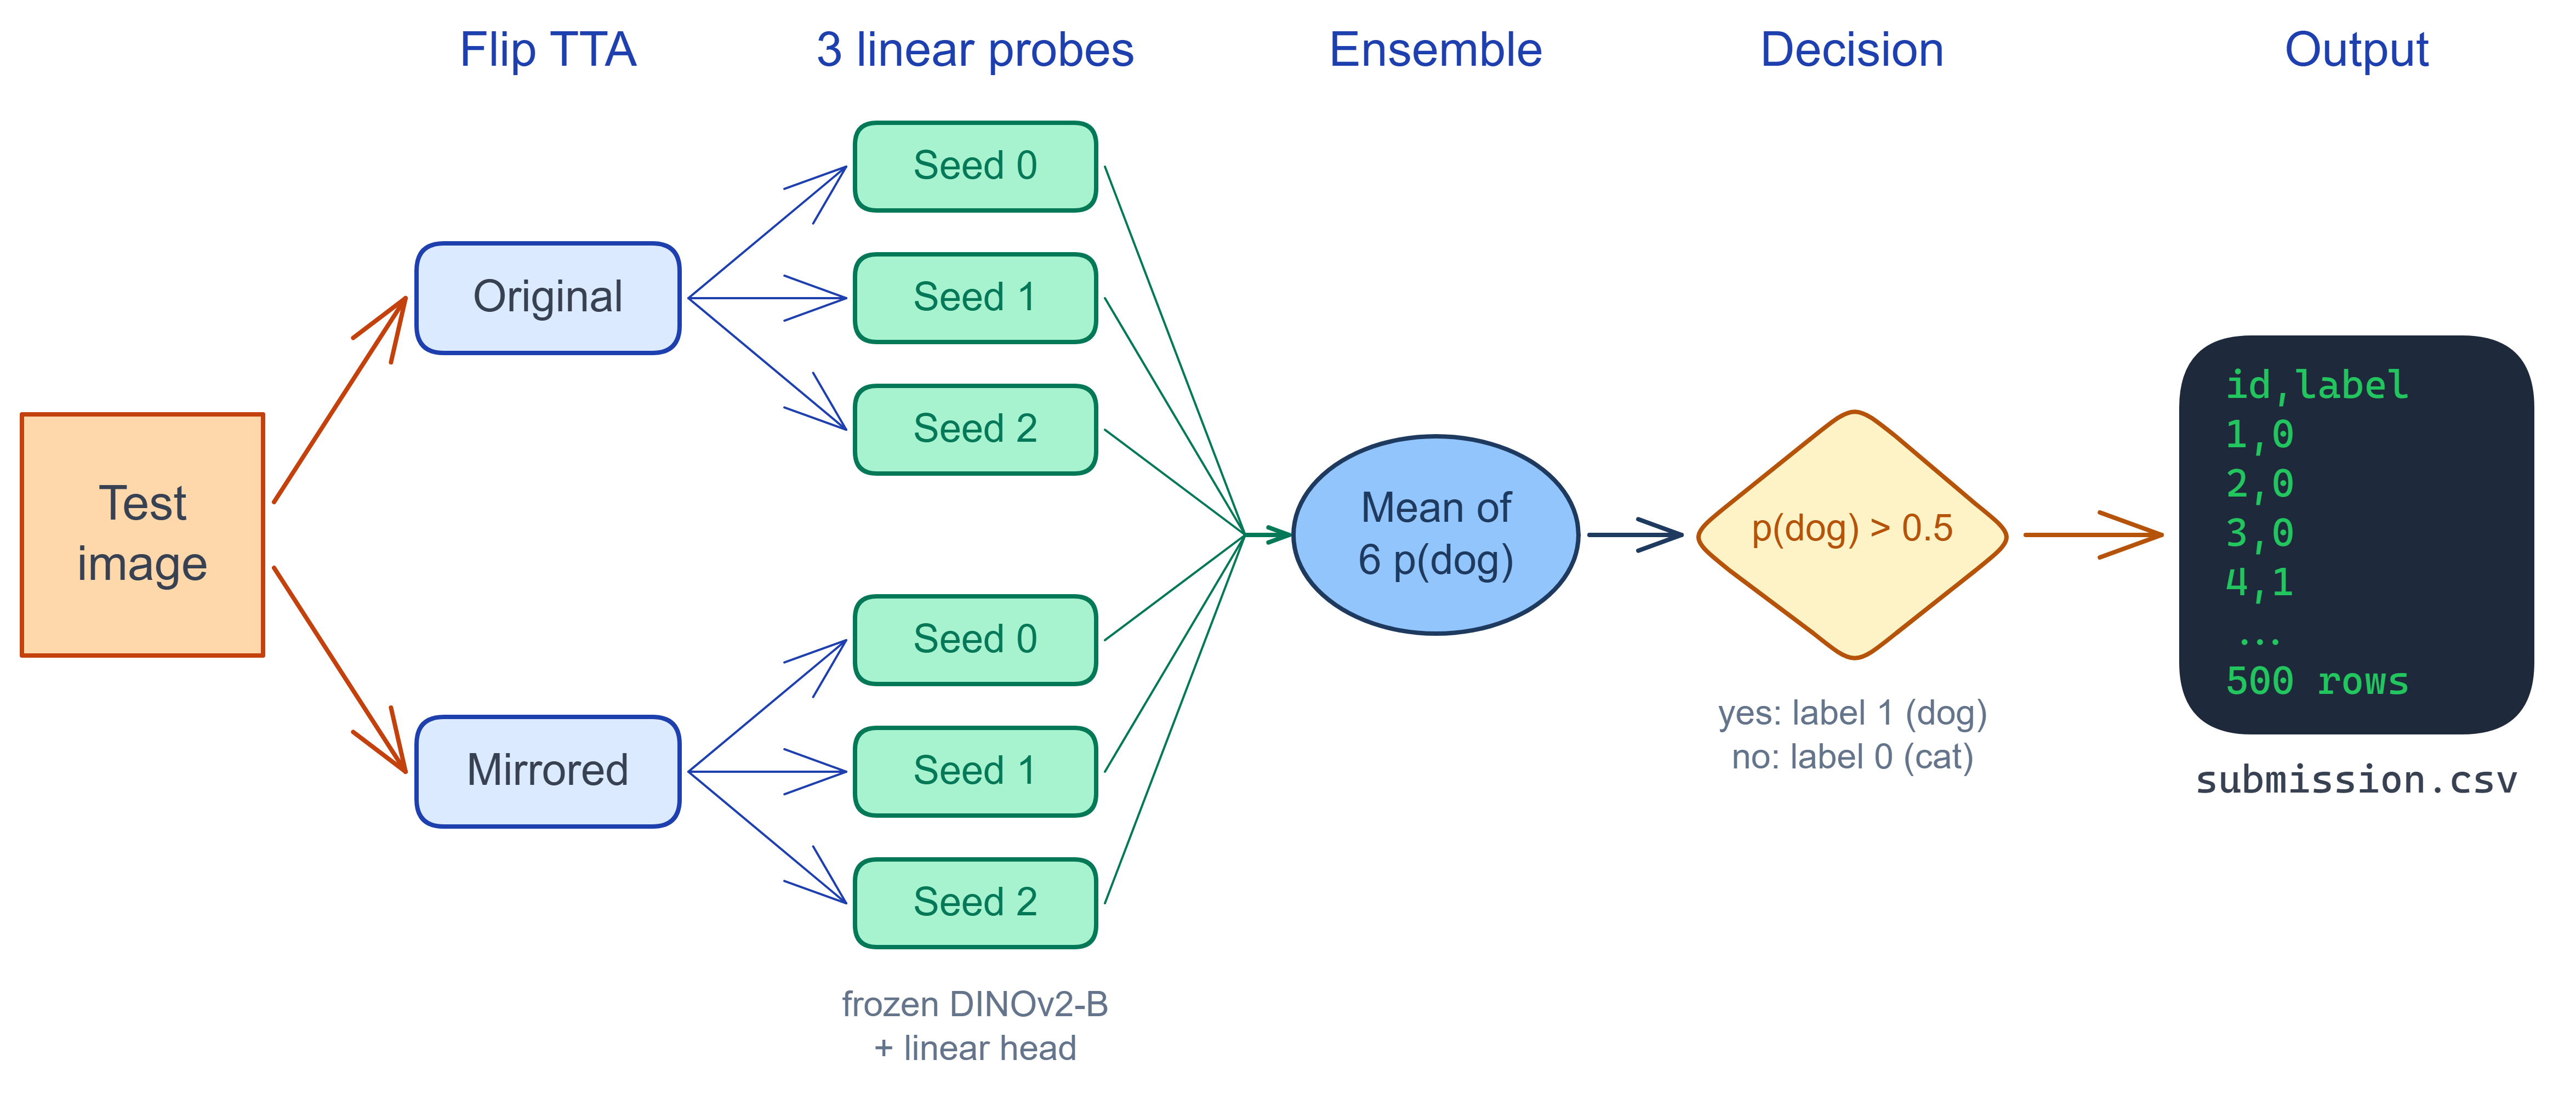
\includegraphics[width=0.9\textwidth]{figures/prediction_pipeline.png}
  \caption{Final prediction procedure.}
  \label{fig:pipeline}
\end{figure}

The model was implemented in Python and PyTorch~\cite{paszke2019pytorch}, with pretrained weights loaded through the timm library~\cite{wightman2019timm}. All code and the saved outputs of every training run are available in the project's GitHub repository, \repo, and Appendix~\ref{app:run} explains how to use it.

% ================================================================== (c)
\section{Choice of Parameters and Settings}\label{sec:c}

\begin{question}
Discuss how you consider and determine the parameters (e.g., learning rate, etc.) / settings of your model as well as your reasons of doing so.
\end{question}

The settings of the final model were chosen in two ways. Where a setting was not expected to change the result much, a standard value from the literature was adopted. For the settings expected to matter most (the learning rate, the training strategy and the initialisation), controlled experiments were run. All comparisons used the last-epoch validation accuracy (\cref{sec:b}). Differences smaller than about 0.1 percentage points (five validation images) were treated as run-to-run variation.

\subsection*{Learning Rate Selection}

The learning rate is an important hyperparameter because it sets how much the model's weights change during training. To study its effect, four backbone learning rates were tested on the pretrained ResNet-50 model with random seed 0: $1 \times 10^{-5}$, $3 \times 10^{-5}$, $1 \times 10^{-4}$ and $3 \times 10^{-4}$. The classification head learning rate was fixed at 0.001. ResNet-50 was chosen for this sweep because it is the fastest of the pretrained models to fine-tune. Each run used the linear-probe-then-fine-tune (LP-FT) strategy~\cite{kumar2022lpft}. The new classification head was first trained alone for one epoch (epoch 0), and the whole network was then fine-tuned for nine epochs. In this report, ``fine-tuned'' and FT always refer to LP-FT.

\Cref{tab:lr,fig:lr} show the resulting validation accuracies. \Cref{fig:lr}a gives the accuracy per epoch, and \cref{fig:lr}b plots the last-epoch accuracy against the backbone learning rate, with the head-only result as a dashed line.

\begin{table}[ht]
  \centering
  \small
  \caption{Effect of the backbone learning rate on ResNet-50 validation accuracy (seed 0).}
  \label{tab:lr}
  \begin{tabular}{@{}lcc@{}}
    \toprule
    Backbone learning rate & After head-only epoch (\%) & Last epoch (\%) \\
    \midrule
    $1 \times 10^{-5}$ & 99.58 & 98.98 \\
    $3 \times 10^{-5}$ & 99.58 & 99.30 \\
    $1 \times 10^{-4}$ & 99.58 & 99.48 \\
    $3 \times 10^{-4}$ & 99.58 & 99.52 \\
    \bottomrule
  \end{tabular}
\end{table}

\begin{figure}[ht]
  \centering
  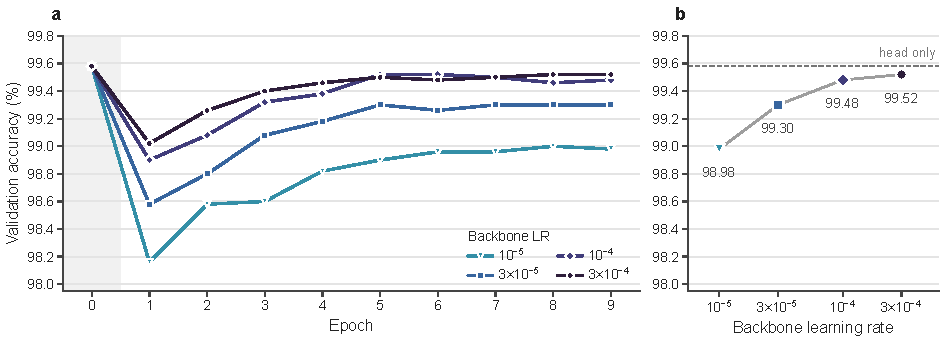
\includegraphics[width=\textwidth]{figures/lr_sweep.pdf}
  \caption{Backbone learning rate sweep on ResNet-50 (seed 0). The grey area marks the head-only epoch.}
  \label{fig:lr}
\end{figure}

Within the tested range, a higher backbone learning rate gave a higher final validation accuracy. All four runs reached \pct{99.58} after the first epoch, because only the classification head was trained in that epoch and the backbone learning rate had no effect yet. Once the backbone was unfrozen, the validation accuracy first dropped and then slowly recovered. Even at the highest learning rate, the final accuracy stayed below the head-only result. This suggests that fine-tuning the pretrained features did not necessarily improve performance on this task.

The sweep has two limitations. First, it used only one seed. The two highest learning rates (\pct{99.48} and \pct{99.52}) differ by only two validation images, which is within the normal variation between runs. Second, the accuracy was still rising at the highest learning rate, so the sweep did not find an optimum. The more important finding is that every fine-tuning run ended below the head-only result, which led to the comparison of training strategies below. The final model does not use a backbone learning rate, because its backbone is frozen. Its head learning rate is discussed under Other Training Settings.

\subsection*{Training Strategy Selection}

Linear probing was then compared with LP-FT on four pretrained backbones (\cref{tab:strategy}). For this comparison, LP-FT used a backbone learning rate of $1 \times 10^{-4}$ for the CNNs, and $5 \times 10^{-5}$ with a layer-wise decay of 0.75 for the vision transformers. For DINOv2-B, linear probing reached \pmpct{99.86}{0.02}, against \pmpct{99.77}{0.02} for LP-FT. Linear probing was also better for ResNet-50, while for ConvNeXt-T and DINOv2-S the two strategies differed by at most 0.04 percentage points (two images).

\begin{table}[ht]
  \centering
  \small
  \caption{Validation accuracy (\%) of linear probing and LP-FT over three seeds, and training time of one run on one GPU.}
  \label{tab:strategy}
  \setlength{\tabcolsep}{5pt}
  \begin{tabular}{@{}llccrr@{}}
    \toprule
    Backbone & Pretraining data & Linear probe & Fine-tuned (LP-FT) & Probe $-$ FT & Time (probe / FT) \\
    \midrule
    ResNet-50  & ImageNet-1k~\cite{deng2009imagenet} & $99.52 \pm 0.03$ & $99.45 \pm 0.01$ & $+0.07$ & 4.6 / 7.9 min \\
    ConvNeXt-T & ImageNet-22k & $99.66 \pm 0.02$ & $99.70 \pm 0.04$ & $-0.04$ & 4.6 / 10.4 min \\
    DINOv2-S   & LVD-142M & $99.71 \pm 0.02$ & $99.73 \pm 0.05$ & $-0.02$ & 4.7 / 9.1 min \\
    DINOv2-B   & LVD-142M & $\mathbf{99.86 \pm 0.02}$ & $99.77 \pm 0.02$ & $+0.09$ & 8.0 / 21.1 min \\
    \bottomrule
  \end{tabular}
\end{table}

\begin{figure}[ht]
  \centering
  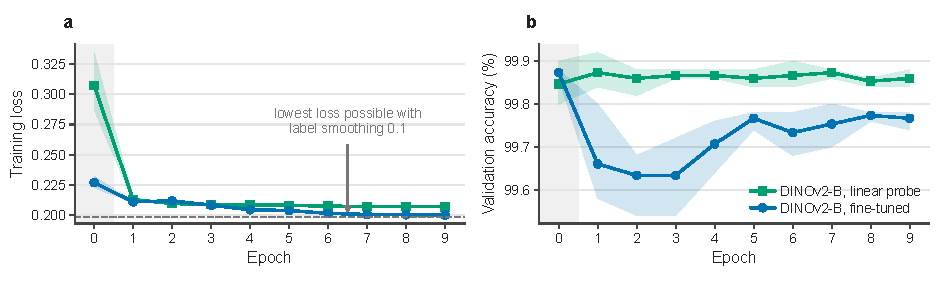
\includegraphics[width=\textwidth]{figures/probe_curves.pdf}
  \caption{Training curves of DINOv2-B for the linear probe and LP-FT. Lines are the mean over three seeds and bands show the spread. The grey area marks the head-only epoch of LP-FT.}
  \label{fig:curves}
\end{figure}

This outcome agrees with the feature-distortion argument of Kumar et al.~\cite{kumar2022lpft}. When pretrained features already separate the classes well, updating the whole network can distort those features and reduce accuracy. ImageNet contains many cat and dog breeds, and DINOv2 was pretrained on 142 million images, so their frozen features already separate the two classes almost perfectly. \Cref{fig:curves}b shows this effect for DINOv2-B. The fine-tuned model reaches \pct{99.87} after its head-only epoch, falls to between \pct{99.63} and \pct{99.66} in the three epochs after the backbone is unfrozen, and recovers only to \pct{99.77} by the last epoch.

Further experiments lowered the backbone learning rate for DINOv2-B fine-tuning to $1 \times 10^{-5}$, which raised validation accuracy to \pmpct{99.87}{0.04}. However, this setting was tested with only two random seeds, and its small gain over linear probing was within the variation across runs. A fine-tuning run with the lighter augmentation of \cref{sec:f} reached \pct{99.82}, again no better than the probe. Fine-tuning thus performed comparably to linear probing, but it updated the whole pretrained network and took 21.1 instead of 8.0 minutes per run. Linear probing was therefore selected as the final training strategy, because it reached similarly high accuracy with fewer trainable parameters and less computation.

\subsection*{Initialisation}

Weight initialisation mattered in two ways, and the larger effect came from the backbone. The scratch CNN, whose weights were randomly initialised with He initialisation~\cite{he2015init}, reached \pct{97.65} after 50 epochs. In contrast, with the default settings, every backbone initialised from pretrained weights exceeded \pct{99.4} within 10 epochs (\cref{sec:f}). Pretrained initialisation was therefore the most important single setting in this project.

The initialisation of the new classification head also mattered. For every pretrained backbone, the original classifier was replaced by a new linear layer with two outputs, and the timm library initialises this layer differently for different architectures. For EfficientNetV2-S, the initial head weights had a standard deviation of 0.41, more than 20 times larger than for the other backbones, and its head-only epoch reached only about \pct{90} validation accuracy. Re-initialising the head from a truncated normal distribution (standard deviation 0.02, zero bias), the same scale as the other backbones, raised the final accuracy of EfficientNetV2-S from \pct{99.12} to \pct{99.64}. The code applies this correction automatically whenever the initial head weights have a standard deviation above 0.05 (\texttt{src/models.py} in the repository). The DINOv2-B head was below this threshold and was not modified.

\subsection*{Other Training Settings}

AdamW~\cite{loshchilov2019adamw} adapts the step size of each parameter as in Adam~\cite{kingma2015adam} and decouples the weight decay from this adaptive update, which makes the regularisation effective at reducing overfitting. It was used with the head learning rate of 0.001 and the weight decay of 0.05 given in \cref{sec:b}.

The head learning rate and the weight decay were not tuned separately for each model. They are common defaults for training a new linear layer with AdamW, and they were used for every pretrained model so that the comparisons in this section differ only in the factor under study. Their suitability for the final model was checked from its training curves (\cref{fig:curves}). The training loss fell to 0.21 within two epochs and to 0.207 by the last epoch, close to the minimum of 0.199 attainable with label smoothing. From the second epoch onwards, the validation accuracy of every seed stayed between \pct{99.82} and \pct{99.92}, a band of five images. This indicates that the head had converged and that a different head learning rate had little room to improve the result.

A batch size of 64 was used to fit the computational demands of fine-tuning DINOv2-B. The same value was kept for the linear probe, so that the two strategies used the same batch size, optimiser and number of epochs and differed mainly in which parameters were updated. The one-epoch warm-up raised the learning rate gradually to avoid large parameter updates early in training, and the cosine decay then lowered it steadily for more stable learning in the final epochs. The flat curves after the second epoch in \cref{fig:curves} show that 10 epochs were sufficient.

Label smoothing (\cref{eq:loss}) and the augmentation pipeline of \cref{sec:a} were kept at standard values, since \cref{sec:f} shows that the pretrained models are far less sensitive to them than the scratch CNN.

Overall, the experiments showed that the pretrained DINOv2-B features were already effective at separating cats and dogs. Keeping the backbone frozen gave strong classification performance without the extra computational cost of full fine-tuning.

% ================================================================== (d)
\section{Validation Accuracy and Test Predictions}\label{sec:d}

\begin{question}
Report the classification accuracy on validation set. Apply the classifier(s) built to the test set. Submit the ``submission.csv'' with the results you obtained.
\end{question}

\subsection*{Validation Results}

The final DINOv2-B classifier, the three-seed ensemble with flip TTA of \cref{fig:pipeline}, was evaluated on the 4,999 validation images. The individual DINOv2-B linear probes reached a mean validation accuracy of \pmpct{99.86}{0.02} without TTA and \pmpct{99.88}{0.02} with TTA (\cref{tab:seeds}). The final three-seed ensemble reached \pct{99.88}, correctly classifying 4,993 of the 4,999 validation images with only six errors.

\begin{table}[ht]
  \centering
  \small
  \caption{Validation accuracy (\%) of the DINOv2-B linear probe and the final ensemble.}
  \label{tab:seeds}
  \begin{tabular}{@{}lcc@{}}
    \toprule
    Model & Without TTA & With flip TTA \\
    \midrule
    Seed 0 & 99.88 & 99.90 \\
    Seed 1 & 99.86 & 99.88 \\
    Seed 2 & 99.84 & 99.86 \\
    Mean $\pm$ standard deviation & $99.86 \pm 0.02$ & $99.88 \pm 0.02$ \\
    \midrule
    Final three-seed ensemble & -- & \textbf{99.88} (4,993 / 4,999) \\
    \bottomrule
  \end{tabular}
\end{table}

The ensemble accuracy of \pct{99.88} equals the mean of the single probes with TTA, so ensembling did not improve accuracy. The three probes share the same frozen features and differ only in the random initialisation of the 1,538 head parameters, the order of the training images and the random augmentations, and their predictions agree on all 500 test images. The ensemble was still kept because it avoids picking a single seed based on its validation accuracy, which would be an optimistic choice. Averaging different architectures did not help either. An ensemble of the DINOv2-B probes with the fine-tuned DINOv2-S and ConvNeXt-T models reached \pct{99.84}, below DINOv2-B alone, because the weaker models dilute the predictions of the strongest one.

\begin{table}[ht]
  \centering
  \small
  \caption{Confusion matrix of the final DINOv2-B classifier on the validation set.}
  \label{tab:confusion}
  \begin{tabular}{@{}lccc@{}}
    \toprule
    Actual class & Predicted cat & Predicted dog & Recall (\%) \\
    \midrule
    Cat & 2,495 & 4     & 99.84 \\
    Dog & 2     & 2,498 & 99.92 \\
    \midrule
    Precision (\%) & 99.92 & 99.84 & \\
    \bottomrule
  \end{tabular}
\end{table}

\Cref{tab:confusion} gives the confusion matrix of the final ensemble. Four of the 2,499 cat images were predicted as dogs and two of the 2,500 dog images as cats, so the classifier performed consistently well on both classes. The six misclassified images are analysed in \cref{sec:e}.

\subsection*{Test Classification Results}

The final classifier was then applied to the 500 unlabelled test images with the procedure of \cref{fig:pipeline}. It predicted 259 images as dogs and 241 as cats. The labels were written to \texttt{submission.csv}, which follows the format of the provided sample file, with the image ID and the predicted label (1 for dog, 0 for cat).

Since the test set has no ground-truth labels, its accuracy cannot be measured, so the reported accuracy of \pct{99.88} refers to the validation set.

% ================================================================== (e)
\section{Analysis of Test-Set Predictions}\label{sec:e}

\begin{question}
Analyse some correctly and incorrectly classified (if any) samples in the test set. Select 1-2 cases to discuss the strength and weakness of the model.
\end{question}

Because the test predictions cannot be scored (\cref{sec:d}), all 500 were checked by eye, and no incorrect prediction was found. The correct cases below therefore come from the test set, and the incorrect cases are the six misclassified validation images, which do have labels. As in \cref{sec:b}, a value of \pdog\ above 0.5 is a dog prediction. The classifier was rarely uncertain, since only three of the 500 test images have \pdog\ between 0.2 and 0.8.

\subsection*{Correctly Classified Test Cases}

\Cref{fig:testcases}a shows the six least confident test predictions, and \cref{fig:testcases}b shows the three most confident predictions for each class. Because of label smoothing (\cref{eq:loss}), most confident predictions lie near 0.05 and 0.95. Two cases show the strength and the weakness of the model.

\textbf{Test image 26 (strength).} This image shows a cat beside a scratching post on a patterned rug. It was correctly classified with \pdog\ = 0.02, the second most confident of the 500 predictions. The rug, the post and the date stamp in the corner did not distract the model. 

\textbf{Test image 469 (weakness).} This small and blurry photograph of merle puppies is only $108 \times 82$ pixels in size. Its shorter side was therefore enlarged about 2.7 times to reach the 224-pixel input. It was correctly classified, but with \pdog\ = 0.65 it is the least confident of the 500 predictions. At this resolution, the fine detail that normally separates the two classes is missing.

The other uncertain test images in \cref{fig:testcases}a show similar difficulties. Image 216 (\pdog\ = 0.25) shows cats behind cage bars with yellow text overlaid. Image 47 (0.80) shows puppies far away in a basket, seen through a chain-link fence, and image 179 (0.83) shows a greyhound, whose slim body is unusual for a dog. In image 293 (0.15), the cat is small and sits in a toy pram beside a child, and image 342 (0.14) is a small, dark photograph with low contrast. All of these predictions were judged to be correct.

\begin{figure}[ht]
  \centering
  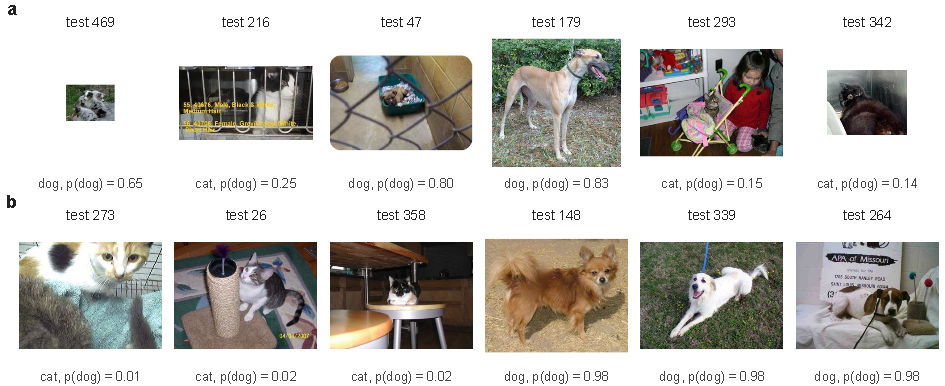
\includegraphics[width=\textwidth]{figures/test_cases.pdf}
  \caption{Test images with the final classifier's predictions.}
  \label{fig:testcases}
\end{figure}

\subsection*{Misclassified Validation Images}

\Cref{fig:errors}a shows the six validation images misclassified by the final classifier, and \cref{fig:errors}b shows the six least confident correct predictions.

Four of the six errors are caused by the dataset rather than by the model, because these images do not clearly show a single cat. The images \texttt{cat.7920} (\pdog\ = 0.93) and \texttt{cat.9882} (0.92) show a dog and a cat together, so a dog prediction is a reasonable answer. The image \texttt{cat.7377} (0.85) is a portrait of a man with no animal in it, and \texttt{cat.3672} (0.67) is a group of people with a small cat on a table. Only the two dog images are genuine mistakes, and both predictions are uncertain. The image \texttt{dog.7164} (0.39) shows a white puppy lying upside down on a person's lap beneath a caption, and \texttt{dog.11248} (0.49) is a strip of only $99 \times 37$ pixels showing several animals.

Most of the six errors therefore come from the labels and the single-label format, which suggests that the validation accuracy of \pct{99.88} is close to the limit that this dataset allows. \Cref{fig:errors}b supports this, since several of the least confident correct predictions also show a cat and a dog in the same image. In contrast, the scratch CNN makes between 114 and 123 validation errors per seed, including many clear photographs of a single animal.

\begin{figure}[ht]
  \centering
  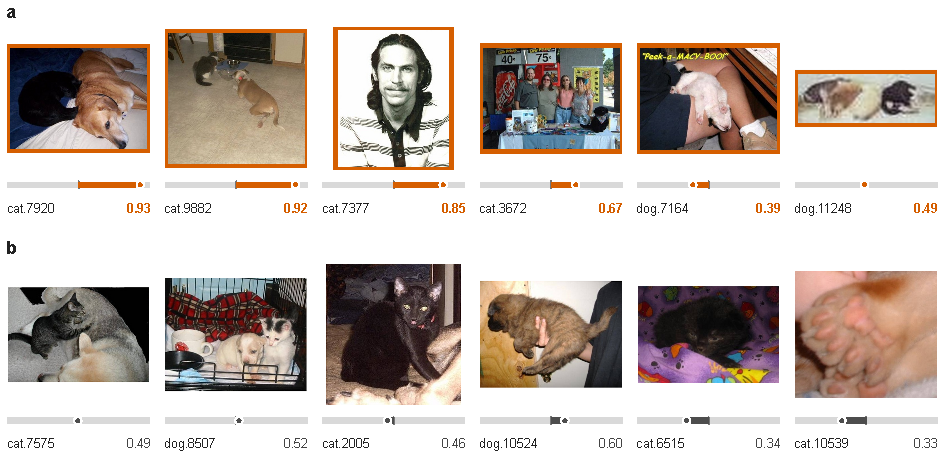
\includegraphics[width=\textwidth]{figures/errors_final_val.pdf}
  \caption{Validation images analysed for the final classifier, (a) misclassified, most confident first, and (b) the least confident correct predictions. The file name gives the dataset label. The bar under each image runs from \pdog\ = 0 (cat, left) to 1 (dog, right), and its coloured segment runs from the 0.5 threshold to the prediction.}
  \label{fig:errors}
\end{figure}

\subsection*{Where the Models Look}

\Cref{fig:gradcam} uses Grad-CAM~\cite{selvaraju2017gradcam} to compare the image regions that influence the final model and the scratch CNN. The maps are computed for the last transformer block of the DINOv2-B linear probe and the last convolutional block of the scratch CNN (seed 0 for both). They are shown for the four validation images that the final model is most confidently wrong about, one easy cat, one easy dog and the two test images it is least sure about. Each map is rescaled to the range 0 to 1 within its own image, so it compares locations within an image, not strength across images.

On the easy dog image (\texttt{dog.828}) and on test image 469, the strongest DINOv2-B responses fall on the animal's head. On \texttt{cat.7920}, they lie mostly around the dog's muzzle and not on the black cat, which agrees with the dog prediction. On \texttt{cat.7377}, which contains no animal, they fall on the man's nose and moustache, although the model must still choose one of the two classes. The scratch CNN responds to one broad region instead. On test image 469, this region lies mostly on the background above the puppies, even though its dog prediction is confident. This suggests that its decision is less closely tied to the animal.


\begin{figure}[ht]
  \centering
  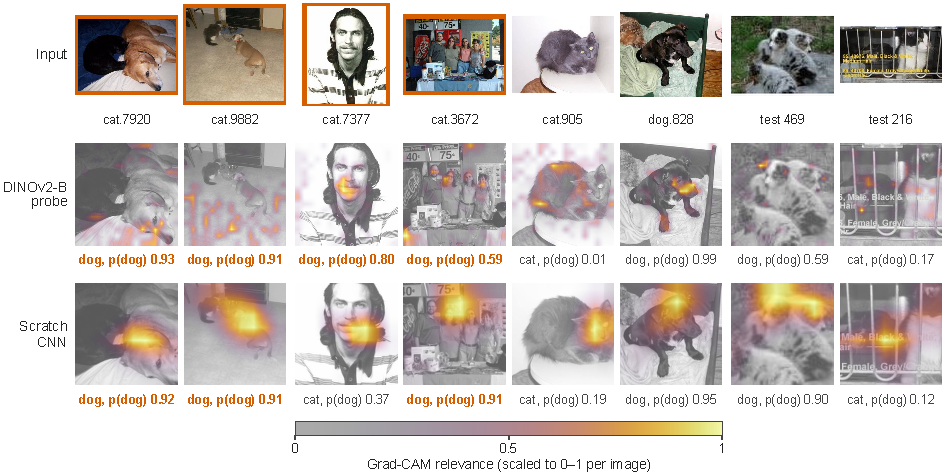
\includegraphics[width=\textwidth]{figures/gradcam.pdf}
  \caption{Grad-CAM maps of the final model and the scratch CNN. The top row shows the whole image, and the lower rows show the centre crop that each model receives with the map for the predicted class. The labels give the prediction of the single seed-0 model without TTA, so they differ slightly from those of the final classifier. Orange labels are wrong.}
  \label{fig:gradcam}
\end{figure}

\subsection*{Strengths and Weaknesses}

The strength of the model is that it is confident and correct on ordinary photographs, whatever the pose, breed or background. Its confidence falls when the animal is small in the frame, blocked by bars or a fence, low in resolution or blurred, overlaid with text, or of an unusual breed. The model also has a structural weakness, i.e.\ its softmax output must always choose between cat and dog, so it cannot recognise an image that contains both animals or neither of them. It can even be confident on such images, as the predictions of 0.93 for \texttt{cat.7920} (a cat and a dog) and 0.85 for \texttt{cat.7377} (no animal) show.

% ================================================================== (f)
\section{Effect of Model Choice and Data Processing}\label{sec:f}

\begin{question}
Discuss how different choice of models and data processing may affect the project in terms of accuracy on validation set.
\end{question}

\subsection*{Choice of Model}

The models compared here were introduced in \cref{sec:b}, and the baselines are described below. The two classical baselines were trained on HOG features and a colour histogram extracted from $128 \times 128$ images. One used a linear SVM, and the other used an RBF SVM after principal component analysis. The scratch CNN has five convolutional blocks and 2.35 million parameters. It was trained for 50 epochs with SGD and a one-cycle learning rate schedule~\cite{smith2019onecycle}.

\Cref{fig:ladder,tab:models} compare all models. The HOG baselines are deterministic and were run once.

The choice of model had a very large effect at the low end of the comparison. The HOG baselines reached only \pct{68.29} and \pct{80.06}, because hand-crafted features describe edges and colours but not the appearance of the animals. Learning the features raised the accuracy to \pct{97.65} with the scratch CNN. Every pretrained model then exceeded \pct{99.4}, between 1.8 and 2.2 points above the scratch CNN.

Among the pretrained models, the differences were much smaller, and pretraining mattered more than architecture size. The four fine-tuned backbones with 20 to 28 million parameters differ by only 0.28 points, and their accuracy does not increase with size. Excluding ResNet-50, they lie within 0.09 points of each other. DINOv2-B has about four times as many parameters as DINOv2-S but added only 0.15 points as a linear probe. Instead, the accuracy follows the amount of pretraining data. It lies between \pct{99.45} and \pct{99.52} for ImageNet-1k, between \pct{99.64} and \pct{99.70} for ImageNet-21k and 22k, and between \pct{99.71} and \pct{99.86} for the 142 million images of DINOv2. However, each backbone was tested with only one set of pretrained weights, so this trend cannot be fully separated from the architecture.

As shown in \cref{sec:c}, the training strategy mainly changed the training time, with no clear gain in accuracy from fine-tuning (\cref{tab:models}).

\begin{figure}[ht]
  \centering
  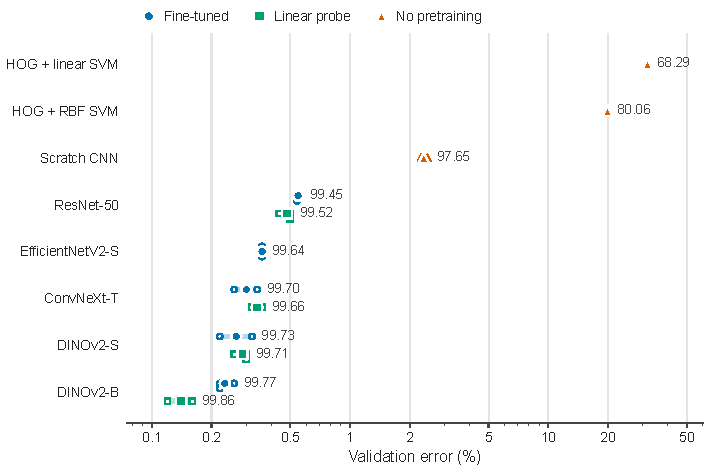
\includegraphics[width=0.78\textwidth]{figures/model_ladder.pdf}
  \caption{Validation error of all Dogs vs.\ Cats models (logarithmic axis). Large markers are the mean over the seeds, small open markers are individual seeds, the pale bars show their range and the numbers give the mean validation accuracy (\%).}
  \label{fig:ladder}
\end{figure}

\begin{table}[ht]
  \centering
  \small
  \caption{Validation accuracy (\%) and training time of all Dogs vs.\ Cats models. The final model is shown in bold.}
  \label{tab:models}
  \setlength{\tabcolsep}{5pt}
  \begin{tabular}{@{}lllrcccr@{}}
    \toprule
    Model & Pretraining data & Training & Params (M) & $n$ & Val.\ acc. & With flip TTA & Time (min) \\
    \midrule
    HOG + linear SVM & none & classical & -- & 1 & 68.29 & -- & 4.0 \\
    HOG + RBF SVM & none & classical & -- & 1 & 80.06 & -- & 5.5 \\
    Scratch CNN & none & all layers & 2.35 & 3 & $97.65 \pm 0.09$ & $97.81 \pm 0.14$ & 11.1 \\
    ResNet-50 & ImageNet-1k & FT & 23.51 & 3 & $99.45 \pm 0.01$ & $99.49 \pm 0.06$ & 7.9 \\
    ResNet-50 & ImageNet-1k & probe & 23.51 & 3 & $99.52 \pm 0.03$ & $99.59 \pm 0.02$ & 4.6 \\
    EfficientNetV2-S & ImageNet-21k & FT & 20.18 & 3 & $99.64 \pm 0.00$ & $99.67 \pm 0.03$ & 18.4 \\
    ConvNeXt-T & ImageNet-22k & FT & 27.82 & 3 & $99.70 \pm 0.04$ & $99.71 \pm 0.04$ & 10.4 \\
    ConvNeXt-T & ImageNet-22k & probe & 27.82 & 3 & $99.66 \pm 0.02$ & $99.69 \pm 0.01$ & 4.6 \\
    DINOv2-S & LVD-142M & FT & 21.63 & 3 & $99.73 \pm 0.05$ & $99.73 \pm 0.02$ & 9.1 \\
    DINOv2-S & LVD-142M & probe & 21.63 & 3 & $99.71 \pm 0.02$ & $99.76 \pm 0.02$ & 4.7 \\
    DINOv2-B & LVD-142M & FT & 85.73 & 3 & $99.77 \pm 0.02$ & $99.77 \pm 0.02$ & 21.1 \\
    \textbf{DINOv2-B} & LVD-142M & \textbf{probe} & 85.73 & 3 & $\mathbf{99.86 \pm 0.02}$ & $\mathbf{99.88 \pm 0.02}$ & 8.0 \\
    \bottomrule
  \end{tabular}
\end{table}

\subsection*{Amount of Training Data}

The effect of the amount of training data also depended strongly on the model (\cref{tab:datasize}). It was tested on class-balanced subsets. The scratch CNN improved by 11.09 points between 2,000 and 20,000 training images, and its accuracy was still rising at the largest size. ResNet-50 gained only 0.64 points. ConvNeXt-T and the DINOv2-B probe stayed flat, with changes smaller than 0.1 points. With only 2,000 images, the DINOv2-B probe reached \pct{99.83}, which is higher than the scratch CNN with all 20,000 images. Strong pretraining therefore replaces at least ten times as much labelled data for this task.

\begin{table}[ht]
  \centering
  \small
  \caption{Validation accuracy (\%) against the number of training images.}
  \label{tab:datasize}
  \begin{tabular}{@{}lcccc@{}}
    \toprule
    Model & 2,000 & 5,000 & 10,000 & 20,000 \\
    \midrule
    Scratch CNN             & $86.56 \pm 1.10$ & $94.01 \pm 0.21$ & $96.45 \pm 0.17$ & $97.65 \pm 0.09$ \\
    ResNet-50 (fine-tuned)  & $98.81 \pm 0.03$ & $99.24 \pm 0.03$ & $99.37 \pm 0.02$ & $99.45 \pm 0.01$ \\
    ConvNeXt-T (fine-tuned) & $99.67 \pm 0.06$ & $99.61 \pm 0.05$ & $99.63 \pm 0.08$ & $99.70 \pm 0.04$ \\
    DINOv2-B (linear probe) & $99.83 \pm 0.01$ & $99.86 \pm 0.02$ & $99.89 \pm 0.02$ & $99.86 \pm 0.02$ \\
    \bottomrule
  \end{tabular}
\end{table}

\subsection*{Data Processing}

Data processing mattered most for the scratch CNN, which has no pretrained features to rely on (\cref{tab:augmentation}). Random resized cropping and horizontal flipping raised its accuracy by 3.16 points, from \pct{94.56} to \pct{97.72}. Adding rotation, colour jitter and random erasing to form the default pipeline of \cref{sec:a} gave no further gain at 50 epochs (\pct{97.65}). Neither did the stronger TrivialAugment policy~\cite{muller2021trivialaugment} (\pct{97.50}). Training the default pipeline for 100 epochs reached \pct{97.90}, which suggests that the CNN was still under-trained at 50 epochs with this much augmentation.

The pretrained models were far less sensitive. A lighter pipeline of cropping and flipping, without label smoothing, changed the accuracy of fine-tuned DINOv2-B and ResNet-50 by less than 0.1 points. Flip TTA helped most where training had no augmentation, adding 0.78 points to the scratch CNN, but it added at most 0.07 points to any pretrained model (\cref{tab:models}).

\begin{table}[ht]
  \centering
  \small
  \caption{Effect of training-time augmentation on the scratch CNN (validation accuracy, \%).}
  \label{tab:augmentation}
  \begin{tabular}{@{}lccll@{}}
    \toprule
    Augmentation & Epochs & $n$ & Val.\ acc. & With flip TTA \\
    \midrule
    None (resize and centre crop)                    &  50 & 1 & 94.56 & 95.34 \\
    Random resized crop and flip                     &  50 & 1 & 97.72 & 97.84 \\
    Default (adds rotation, colour jitter, erasing)   &  50 & 3 & $97.65 \pm 0.09$ & $97.81 \pm 0.14$ \\
    Default and TrivialAugment                       &  50 & 1 & 97.50 & 97.56 \\
    Default                                          & 100 & 1 & 97.90 & 98.22 \\
    \bottomrule
  \end{tabular}
\end{table}

% ================================================================== (g)
% This section has several tables and figures in a row, so allow three floats at the top of a page.
\setcounter{topnumber}{3}
\renewcommand{\topfraction}{0.9}

\section{Multi-Class Classification on CIFAR-10}\label{sec:g}

\begin{question}
Apply and improve your classification algorithm to a multi-category image classification problem for Cifar-10 dataset (\url{https://www.cs.toronto.edu/~kriz/cifar.html}). Describe details about the dataset and classification problem that you are solving. Explain how your algorithm can tackle this problem, and what changes you make comparing to solving Dogs vs. Cats problem. Report your results for the testing set of Cifar-10.
\end{question}

\subsection*{Dataset and Problem}

CIFAR-10~\cite{krizhevsky2009cifar} contains 60,000 RGB images of $32 \times 32$ pixels in ten classes: airplane, automobile, bird, cat, deer, dog, frog, horse, ship and truck. Each class has 6,000 images, with 5,000 in the official training set and 1,000 in the official test set. To form a validation set, 500 images per class were held out from the training set, leaving 45,000 images for training. The 10,000 test images were evaluated only once, after the last training epoch. The problem is therefore to assign each small image to exactly one of ten balanced classes.

\subsection*{Approach and Changes from Dogs vs.\ Cats}

The softmax classifier extends directly to this problem, since the linear head only needs ten outputs instead of two. As a baseline, a CIFAR-style ResNet-18 was trained from scratch for 200 epochs. It has a $3 \times 3$ first convolution and no max-pooling layer, so that the small images are not downsampled too early. It was trained with SGD with Nesterov momentum, a learning rate of 0.1 with a 5-epoch warm-up and cosine decay, a weight decay of $5 \times 10^{-4}$, and random cropping with 4-pixel padding and horizontal flipping.

To improve on this baseline, the Dogs vs.\ Cats pipeline was reused with three pretrained backbones (DINOv2-B, ConvNeXt-T and DINOv2-S). For these models, the images were upsampled from $32 \times 32$ to $224 \times 224$ pixels. \Cref{tab:cifarchanges} lists what changed between the Dogs vs.\ Cats model and the best of these backbones, fine-tuned DINOv2-S (results below).

\begin{table}[ht]
  \centering
  \small
  \caption{Main differences between the final Dogs vs.\ Cats model and the best CIFAR-10 model.}
  \label{tab:cifarchanges}
  \begin{tabularx}{\textwidth}{@{}l X X@{}}
    \toprule
    Setting & Dogs vs.\ Cats & CIFAR-10 \\
    \midrule
    Classes & 2 & 10 \\
    Backbone & DINOv2-B & DINOv2-S \\
    Training strategy & Linear probe, backbone frozen for 10 epochs & LP-FT (\cref{sec:c}), backbone learning rate $5 \times 10^{-5}$, layer-wise decay 0.75 \\
    Input & Photographs resized and cropped to $224 \times 224$ & $32 \times 32$ images upsampled to $224 \times 224$ (bilinear) \\
    Augmentation & Random resized crop, flip, rotation, colour jitter, random erasing & Random crop with 4-pixel padding, flip \\
    Label smoothing & 0.1 & None \\
    Batch size & 64 & 128 \\
    Validation data & Provided validation set & 500 images per class held out from training \\
    Final prediction & Three-seed ensemble with flip TTA & Single run, reported with and without flip TTA \\
    \bottomrule
  \end{tabularx}
\end{table}

\subsection*{Test Results}

\Cref{tab:cifar,fig:cifarg} show the test results. The scratch ResNet-18 reached \pmpct{94.78}{0.25}. The best model, fine-tuned DINOv2-S, reached \pct{98.87}, or \pct{98.93} with flip TTA. This reduces the number of test errors from about 522 to 113, and DINOv2-S needed only 10 epochs (16.9 minutes) instead of the 200 epochs (about 26 minutes) of ResNet-18. The three pretrained models were run with one seed each, but they rank in the same order on the validation set.

\begin{table}[ht]
  \centering
  \small
  \caption{CIFAR-10 test accuracy (\%) of each model.}
  \label{tab:cifar}
  \setlength{\tabcolsep}{5pt}
  \begin{tabular}{@{}lllccll@{}}
    \toprule
    Model & Training & Input & Epochs & $n$ & Test acc. & With flip TTA \\
    \midrule
    ResNet-18 (CIFAR variant) & from scratch & $32 \times 32$ & 200 & 3 & $94.78 \pm 0.25$ & $95.13 \pm 0.09$ \\
    DINOv2-B & linear probe & upsampled to 224 & 10 & 1 & 97.99 & 98.15 \\
    ConvNeXt-T & fine-tuned (LP-FT) & upsampled to 224 & 10 & 1 & 98.69 & 98.70 \\
    \textbf{DINOv2-S} & fine-tuned (LP-FT) & upsampled to 224 & 10 & 1 & \textbf{98.87} & \textbf{98.93} \\
    \bottomrule
  \end{tabular}
\end{table}

\begin{figure}[ht]
  \centering
  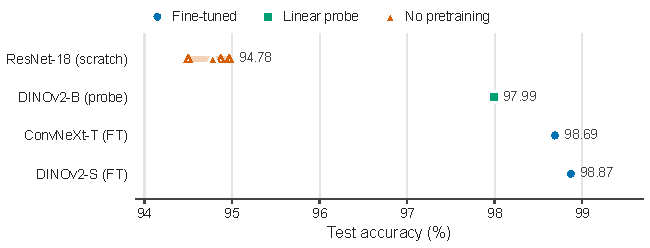
\includegraphics[width=0.78\textwidth]{figures/cifar_g.pdf}
  \caption{CIFAR-10 test accuracy of each model. Colours and markers as in \cref{fig:ladder}.}
  \label{fig:cifarg}
\end{figure}

Unlike on Dogs vs.\ Cats, the frozen linear probe was the weakest of the transfer models here. A likely reason is that upsampled $32 \times 32$ images look very different from the photographs used for pretraining, so the frozen features fit less well and fine-tuning has more to correct. The comparison is not like-for-like, because the probe used DINOv2-B and the fine-tuned models used other backbones. Even so, it suggests that the best strategy depends on how closely the new data resembles the pretraining data.

Cats and dogs are also the hardest CIFAR-10 classes. Their per-class accuracies are about \pct{88.2} and \pct{91.0} for ResNet-18, and \pct{96.4} and \pct{97.4} for DINOv2-S, the two lowest for each model. Confusions between cats and dogs account for 44 of the 113 test errors of DINOv2-S.

% ================================================================== (h)
\section{Class Imbalance in CIFAR-10}\label{sec:h}

\begin{question}
Train the classifier for (g), while some of the classes in Cifar-10 training dataset contains much fewer labelled data. How can you improve your algorithm to tackle the data unbalancing issue? Describe and justify at least 2 approaches you use.
\end{question}

\subsection*{Imbalanced Training Set}

The training set was made long-tailed with an exponential profile. Class $c$ (from 0 to 9) keeps $n_c = \lfloor 4500 \, R^{-c/9} \rfloor$ images, where the imbalance ratio $R$ is the size of the largest class divided by the size of the smallest. For $R = 100$, the classes fall from 4,500 images to 45, leaving 11,165 training images. For $R = 10$, they fall from 4,500 to 450, leaving 18,388. The validation and test sets stay balanced, and the model and training settings are those of the scratch ResNet-18 in \cref{sec:g}. The scratch ResNet-18 was used rather than the best model of \cref{sec:g}, because a pretrained backbone brings features learned from large datasets and would therefore be less affected by the imbalance. Training from scratch shows the effect of the imbalance, and of each method against it, more clearly. This also follows the standard long-tailed CIFAR-10 benchmarks, in which the networks are trained from scratch~\cite{cao2019ldam,menon2021logitadjustment}.

Imbalance reduced the test accuracy of the ResNet-18 trained with plain cross-entropy from \pct{94.78} to \pct{88.89} at $R = 10$ and \pct{74.12} at $R = 100$. Cross-entropy averages over the training images, so the model learns the training distribution and favours the frequent classes. To show where the errors occur at $R = 100$, the head, medium and tail accuracies are the mean accuracies of the three largest classes (4,500 to 1,617 training images), the four middle classes (969 to 208) and the three smallest classes (125 to 45). With cross-entropy, the head still reached \pct{94.5}, but the tail reached only \pct{52.1}. Two main approaches were tested against this baseline, and both improved on it (\cref{tab:imbalance,fig:cifarh}).

\subsection*{Approach 1: Class-Balanced Weights with Deferred Re-Weighting}

The first approach weights the loss of each class by the inverse of its effective number of samples~\cite{cui2019classbalanced}. This number accounts for the overlap between similar images, so extra samples of a large class count for less. With hyperparameter $\beta$, the weight of class $c$ is
\begin{equation}
  w_c \propto \frac{1-\beta}{1-\beta^{\,n_c}},
  \label{eq:cb}
\end{equation}
and with $\beta = 0.9999$ the rarest class has about 81 times the weight of the largest class at $R = 100$. The weights were switched on only for the last \pct{20} of the epochs, a schedule known as deferred re-weighting (DRW)~\cite{cao2019ldam}. Training therefore has two stages. For the first 160 epochs, the model trains normally without any rebalancing, which lets it learn general features from all of the images. For the last 40 epochs, the weights shift the decision boundaries towards the frequent classes, which gives the rare classes more room. At $R = 100$, this raised the test accuracy to \pmpct{76.05}{0.28} and the tail accuracy from \pct{52.1} to \pct{56.9}. At $R = 10$, its gain of 0.44 points is within the variation across seeds.

\subsection*{Approach 2: Logit Adjustment}

The second approach is the logit-adjusted loss~\cite{menon2021logitadjustment}. During training, a class-dependent offset based on the class prior $\pi_c = n_c / \sum_k n_k$ is added to each logit $z_c$,
\begin{equation}
  \mathcal{L} = -\log \frac{e^{z_y + \tau \log \pi_y}}{\sum_{c} e^{z_c + \tau \log \pi_c}},
  \label{eq:la}
\end{equation}
with $\tau = 1$. The offsets are used only during training, and at test time the model predicts from the unadjusted logits $z_c$. Because $\log \pi_c$ is most negative for the rare classes, an image of the rarest class at $R = 100$ must beat the largest class by a logit margin of $\log 100 \approx 4.6$ to be classified correctly during training, so rare classes keep a relatively large margin. Unlike a weighted loss, the adjustment also directly compensates for the prior that cross-entropy would otherwise learn. It gave the best results at both ratios, with \pmpct{78.53}{0.51} at $R = 100$ and \pmpct{89.86}{0.13} at $R = 10$. At $R = 100$, the tail accuracy rose from \pct{52.1} to \pct{65.1}, while the head accuracy fell by only 0.7 points. For example, the accuracy on the truck class, which has 45 training images, rose from \pct{47.3} to \pct{64.7}.

\begin{table}[ht]
  \centering
  \small
  \caption{Test accuracy (\%) on long-tailed CIFAR-10 with ResNet-18.}
  \label{tab:imbalance}
  \setlength{\tabcolsep}{5pt}
  \begin{tabular}{@{}lclcccclc@{}}
    \toprule
    & & \multicolumn{4}{c}{$R = 100$} & & \multicolumn{2}{c}{$R = 10$} \\
    \cmidrule{3-6}\cmidrule{8-9}
    Method & $n$ & Overall & Head & Medium & Tail & & Overall & Tail \\
    \midrule
    Cross-entropy (baseline)        & 3 & $74.12 \pm 0.15$ & 94.5 & 75.4 & 52.1 & & $88.89 \pm 0.12$ & 85.5 \\
    Focal loss ($\gamma = 1$)       & 1 & 73.53            & 94.6 & 75.4 & 50.0 & & 89.01            & 85.6 \\
    Class-balanced re-sampling      & 1 & 69.24            & 94.3 & 71.9 & 40.6 & & 88.85            & 85.2 \\
    Class-balanced weights + DRW    & 3 & $76.05 \pm 0.28$ & 94.3 & 76.7 & 56.9 & & $89.33 \pm 0.45$ & 86.7 \\
    \textbf{Logit adjustment} ($\tau = 1$) & 3 & $\mathbf{78.53 \pm 0.51}$ & 93.8 & 77.1 & \textbf{65.1} & & $\mathbf{89.86 \pm 0.13}$ & \textbf{88.3} \\
    \bottomrule
  \end{tabular}
\end{table}

\begin{figure}[ht]
  \centering
  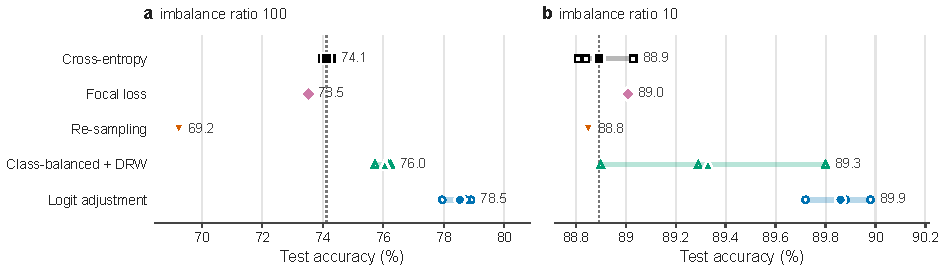
\includegraphics[width=\textwidth]{figures/cifar_h.pdf}
  \caption{Test accuracy on long-tailed CIFAR-10 for imbalance ratios of (a) 100 and (b) 10. The dotted line marks plain cross-entropy, and the two panels have different axis ranges. Markers as in \cref{fig:ladder}.}
  \label{fig:cifarh}
\end{figure}

\subsection*{Other Methods and Comparison}

Two further methods were tested with one seed each. Focal loss~\cite{lin2017focal} with $\gamma = 1$ focuses on hard examples without using the class frequencies, and it gave no improvement at $R = 100$ (\pct{73.53}). Class-balanced re-sampling was worse than the baseline at $R = 100$ (\pct{69.24}). The rarest class has only 45 images, so each of them is drawn about 25 times per epoch, 100 times as often as an image of the largest class. The model therefore probably memorises these few images instead of learning from them. This is consistent with the idea behind DRW, which applies rebalancing only in the last part of training.

The gains in \cref{tab:imbalance} come almost entirely from the rare classes, since the head accuracy stays near \pct{94} for every method. Logit adjustment was the most effective approach, and it requires only one extra line in the loss function. The values of $\beta$ and $\tau$ were not tuned, so these results do not depend on any selection using the test set.

% ================================================================== references
\clearpage
\phantomsection
\addcontentsline{toc}{section}{References}
\bibliographystyle{unsrtnat}
\bibliography{references}

% ================================================================== appendices
\clearpage
\appendix
\renewcommand{\thesection}{\Alph{section}}
\crefname{section}{Appendix}{Appendices}

\section{Code and Reproducibility}\label{app:run}

All code, settings and results of this project are available in the GitHub repository \repo. Its \texttt{README.md} gives step-by-step instructions for two ways of reproducing the results.
\begin{itemize}
  \item \textbf{Quick check (no GPU, about 5 minutes).} Three commands rebuild \texttt{submission.csv} and every result table and figure of the report from the saved outputs of the training runs.
  \item \textbf{Retraining the best models (one NVIDIA GPU, about one hour).} This retrains the final Dogs vs.\ Cats ensemble, fine-tuned DINOv2-S on CIFAR-10 and ResNet-18 with logit adjustment on long-tailed CIFAR-10, and lists the values that the new runs should reach.
\end{itemize}
\Cref{tab:repo} lists the main parts of the repository. Every other run in the report can also be repeated, because the exact settings of each run are stored in its \texttt{args.json} file.

\begin{table}[ht]
  \centering
  \small
  \caption{Main contents of the GitHub repository.}
  \label{tab:repo}
  \begin{tabularx}{\textwidth}{@{}l >{\raggedright\arraybackslash}X@{}}
    \toprule
    Path & Contents \\
    \midrule
    \texttt{src/train.py} & Dogs vs.\ Cats training and evaluation, one model and one seed per run (linear probe or LP-FT, flip TTA, per-run predictions) \\
    \texttt{src/models.py}, \texttt{src/data.py} & Model definitions (scratch CNN, pretrained backbones, head initialisation check), datasets, pre-processing and augmentation \\
    \texttt{src/classical.py} & HOG and colour histogram features with linear and RBF SVMs \\
    \texttt{src/cifar.py} & CIFAR-10 and long-tailed CIFAR-10 experiments (parts (g) and (h)) \\
    \texttt{scripts/} & Pre-resizing, weight download, ensembling, job queue, and the scripts that make every table and figure of the report \\
    \texttt{jobs/} & Command-line arguments of all 106 neural network runs, one run per line \\
    \texttt{runs/} & Saved outputs of all 108 runs: settings (\texttt{args.json}), metrics with per-epoch history (\texttt{metrics.json}), validation and test predictions, and log files \\
    \texttt{report/} & Report figures and tables, and the LaTeX source of this report \\
    \texttt{requirements.txt} & Python packages apart from PyTorch \\
    \bottomrule
  \end{tabularx}
\end{table}

Three further points matter for reproducing the results. First, the course dataset is not included, because it is not ours to redistribute. It has to be placed in a folder \texttt{datasets/}, as described in the \texttt{README.md}. Second, model checkpoints are not included because of their size, so results that need a trained model, such as the Grad-CAM maps, can only be recomputed after retraining. Third, all 108 runs of this report were trained on a Linux server with four NVIDIA RTX 3090 GPUs (24 GB each), one run per GPU, with Python 3.11, PyTorch 2.11.0, CUDA 12.8 and bfloat16 mixed precision, and took about 15 GPU-hours in total. Any recent PyTorch 2.x release works with the code. GPU computations are not fully deterministic, so a retrained run can differ slightly from the saved one (Section~\ref{sec:b}).

\end{document}
